\documentclass[11pt,a4paper]{article}

\usepackage[utf8]{inputenc}
\usepackage[T1]{fontenc}
\usepackage[french]{babel}
\usepackage{geometry}
\geometry{margin=2.5cm}
\usepackage{graphicx}
\usepackage{booktabs}
\usepackage{tabularx}
\usepackage{hyperref}
\usepackage{enumitem}
\usepackage{xurl}
\usepackage{setspace}
\setstretch{1.12}
\setlist{itemsep=0.25em,topsep=0.4em}
\hypersetup{colorlinks=true,linkcolor=black,urlcolor=blue,breaklinks=true}
\Urlmuskip=0mu plus 1mu
\sloppy

\title{RESFLOW\\Réservation de ressources d'un établissement\\Rapport final --- Jalon~4}
\author{Groupe G02\\
NIKIEMA KAFONO ARMAND RAMZIE ARCHAD\\
ZERBO JUDICAEL\\
KOARA Dorianne}
\date{Programmation orientée objet --- 2iE\\Novembre 2026}

\begin{document}
\maketitle
\thispagestyle{empty}

\noindent\textbf{Page d'identification}

\vspace{0.6em}
{\small
\begin{tabularx}{\textwidth}{@{}>{\raggedright\arraybackslash}p{2.4cm} >{\raggedright\arraybackslash}X@{}}
Module & Programmation orientée objet\\
Établissement & 2iE\\
Groupe & G02 (trois membres)\\
Projet & RESFLOW --- réservation de ressources\\
Version livrée & version-1.0\\
Dépôt & lien sous le tableau\\
Tag & version-1.0\\
Membres & NIKIEMA KAFONO ARMAND\\
 & RAMZIE ARCHAD (2E JUMEAU)\\
 & ZERBO JUDICAEL\\
 & KOARA Dorianne\\
\end{tabularx}
}

\vspace{0.4em}
\noindent Dépôt : \url{https://github.com/Ed-sudo-collab/poo-RESFLOW-groupe2}

\noindent Tag : \url{https://github.com/Ed-sudo-collab/poo-RESFLOW-groupe2/tree/version-1.0}

\vspace{0.8em}
\noindent
Ce rapport présente la version finale de RESFLOW. Il explique le besoin, le modèle objet, les choix d'implémentation, la vérification et le bilan. Le code, les essais et le diagramme restent dans le dépôt. Nous n'y recopions pas les classes.

\tableofcontents
\newpage

\section{Besoin, périmètre et fonctionnalités}

Dans un établissement, les salles, les matériels mobiles et les postes de travail sont utilisés par plusieurs personnes au cours de la même journée. Sans registre commun, personne ne sait avec certitude si une salle est libre, qui l'a demandée, ni pour quelles heures. Deux demandes peuvent alors se superposer. Le README du dépôt formule ce constat : l'organisation manuelle produit des conflits d'horaires et une perte de temps.

Un cas suffit à fixer le besoin. Aminata réserve la salle B12 le lundi de 8\,h à 10\,h. Kofi demande ensuite la même salle, le même jour, de 10\,h à 12\,h, alors que la première réservation est encore active. Le programme doit refuser la seconde demande et laisser la salle occupée par Aminata. Si, au contraire, le créneau demandé dure dix heures alors que la salle n'en accepte que quatre, le refus doit intervenir avant toute occupation. C'est ce comportement que la version livrée démontre.

Le périmètre de la version~1.0 tient en trois limites assumées. Le programme est une application console, lancée par compilation puis exécution de \texttt{Main} dans le dossier \texttt{src}. Les données existent seulement en mémoire, le temps d'une exécution : il n'y a pas de base de données. Chaque élément réservable ne porte au plus qu'une réservation active.

Ce qui est réellement codé au tag \texttt{version-1.0} est le suivant. Le catalogue enregistre les éléments et refuse un second exemplaire du même code. La recherche par code distingue un élément trouvé, un code inconnu et un code vide. La réservation n'est acceptée que si l'élément est libre et si la durée ne dépasse pas le maximum du type : quatre heures pour une salle, huit heures pour un matériel mobile, trois heures pour un poste. La libération rend l'élément disponible. La réservation de cours reçoit un jour, une heure de début et une heure de fin, de sorte que le mercredi de 14\,h à 16\,h est bien enregistré avec ces bornes. L'historique conserve les réservations acceptées pendant la démonstration. Le programme principal affiche, pour chaque scénario, le résultat attendu, le résultat obtenu et un verdict.

Ce qui n'est pas codé, et que nous ne présentons que comme suite possible, comprend un rôle d'administrateur, un menu saisi au clavier, l'enregistrement des données après l'arrêt du programme, et l'usage simultané depuis plusieurs postes. Le README évoque aussi, dans la description générale du système, l'ajout ou le retrait de ressources par un administrateur : la version livrée ne réalise pas cette gestion. Elle se limite au catalogue construit dans la démonstration et aux règles de réservation.

Le parcours d'une demande réussie, tel que la démonstration le déroule, éclaire ce périmètre. La salle B12 est d'abord placée dans le catalogue avec un projecteur et un poste. Elle est libre. Une demande de 8\,h à 10\,h, soit deux heures, est inférieure au maximum de quatre heures : elle est acceptée, la salle devient indisponible, et la réservation est versée dans l'historique. Une demande concurrente est alors refusée. Après libération, la même salle peut de nouveau être réservée. Le projecteur, lui, accepte un créneau de cinq heures, parce que son maximum est de huit heures. Le poste accepte un créneau de deux heures, sous son maximum de trois heures. Aucune de ces étapes n'écrit dans un fichier ni n'attend une saisie : elles s'enchaînent dans une seule exécution.

\section{Modèle objet et invariants}

Le diagramme de classes se trouve dans \texttt{docs/Diagrammes de classes.png}. Sa source est \texttt{docs/diagramme.puml}. Il est organisé autour d'un contrat, d'une hiérarchie courte et de quelques associations.

L'interface \texttt{Reservable} fixe ce que tout élément réservable expose : son code, sa disponibilité, une tentative de réservation, une libération, sa durée maximale, la réservation active et un affichage. La classe abstraite \texttt{Ressource} implémente ce contrat pour les objets qui partagent un code, un nom, un indicateur de disponibilité et au plus une réservation active. \texttt{Salle} et \texttt{MaterielMobile} en héritent, parce qu'une salle et un matériel mobile sont des ressources. Elles se distinguent par leurs attributs (capacité d'une part, numéro de série et catégorie d'autre part) et par la durée maximale.

\texttt{PosteTravail} implémente \texttt{Reservable} sans hériter de \texttt{Ressource}. Un poste peut être réservé comme une salle, mais ce n'est ni une salle ni un matériel mobile. Le faire hériter de \texttt{Ressource} aurait imposé un type de ressource qu'il n'est pas. L'interface suffit à le placer dans le même catalogue et dans les mêmes essais. Sa durée maximale est de trois heures. Le README écarte explicitement l'autre solution, qui aurait été de recopier les règles de réservation dans chaque classe concrète.

\texttt{Utilisateur} porte un numéro, un nom et une adresse électronique. \texttt{Creneau} porte un numéro, un jour, une heure de début et une heure de fin, et en déduit la durée. \texttt{Reservation} relie un numéro, un élément réservable, un utilisateur et un créneau. Sans ces trois parties, la réservation ne décrit plus qui occupe quoi et quand. \texttt{CatalogueReservable} regroupe les éléments. \texttt{HistoriqueReservations} regroupe les réservations acceptées. \texttt{ServiceReservation} transmet la tentative de réservation et permet de comparer l'état avant et après un échec. \texttt{ReservationCours} fabrique le créneau d'un cours puis passe par ce service.

Lorsque le programme principal tient une salle, un projecteur ou un poste dans une variable de type \texttt{Reservable}, l'appel est le même. La durée maximale et l'affichage dépendent de l'objet réel. C'est le polymorphisme utilisé dans les essais. Le diagramme rend cette relation visible : \texttt{Salle} et \texttt{MaterielMobile} spécialisent \texttt{Ressource}, tandis que \texttt{PosteTravail} rejoint le même contrat par une autre flèche. \texttt{Reservation} pointe vers l'élément réservé, vers l'utilisateur et vers le créneau. Le catalogue et l'historique pointent vers des collections, pas vers un seul objet. Cette lecture suffit à retrouver, sans le code, quelles données voyagent ensemble lors d'une réservation.

Chaque invariant ci-dessous est une règle observée sur la version livrée, suivie de ce qui se passe si on tente de la violer.
\begin{enumerate}
\item L'heure de fin d'un créneau est strictement supérieure à l'heure de début. Si l'on demande un créneau dont la fin n'est pas après le début, le programme refuse la création et aucun créneau n'est produit.
\item Le code et le nom d'une ressource ne sont pas vides à la création. Si l'un des deux manque, la construction est refusée et aucune ressource n'entre dans le catalogue.
\item La durée acceptée ne dépasse pas la durée maximale de l'élément. Si une salle est demandée de 8\,h à 18\,h, soit dix heures pour un maximum de quatre, la réservation est refusée et la salle reste disponible, sans réservation active.
\item Tant qu'une réservation est active, l'élément n'est pas disponible. Si une seconde demande arrive sur cette salle, elle est refusée et la première réservation demeure.
\item Après une libération, l'élément est de nouveau disponible et n'a plus de réservation active. Une nouvelle demande conforme peut alors être acceptée, comme le montre l'essai qui réserve de nouveau la salle après libération.
\item Le code est unique dans le catalogue. Si l'on ajoute une seconde salle portant le code déjà présent, l'ajout est refusé et la taille du catalogue ne change pas.
\item Un échec de réservation ne modifie ni la disponibilité ni la réservation active. Si la demande est refusée, la comparaison avant/après confirme que l'état est resté le même.
\item Une réservation de cours exige un jour non vide et des heures séparées. Si le jour est vide, la demande est refusée et la salle reste libre. Si le jour est mercredi et les heures 14 et 16, le créneau enregistré porte ces trois informations.
\end{enumerate}

Ces huit règles ne sont pas de simples commentaires. Chacune correspond à un essai de la section~\ref{sec:verif}. L'invariant sur les heures du créneau est celui qui rejette une fin égale au début. L'invariant de durée est celui qui refuse dix heures sur une salle. L'invariant d'occupation est celui qui refuse la demande de Kofi tant qu'Aminata n'a pas libéré la salle. L'invariant d'unicité est celui qui bloque le second code identique. L'invariant d'échec sans mutation est vérifié à part, en comparant l'état d'avant et l'état d'après. Le modèle et les essais décrivent donc la même discipline : une règle n'est retenue que si la démonstration peut la mettre en défaut et constater le refus.

\section{Choix d'implémentation et robustesse}

Nous avons retenu une interface et une classe abstraite pour ne pas recopier les mêmes contrôles. \texttt{Reservable} permet au programme principal, au catalogue et à la réservation de manipuler un seul type. \texttt{Ressource} regroupe, pour la salle et le matériel mobile, le code, le nom, la disponibilité et la réservation active, ainsi que le refus si la durée est trop longue ou si l'élément est déjà pris. Les classes filles ne précisent que ce qui change. Recopier ces règles dans chaque classe aurait suffi pour deux types, mais chaque nouvel élément aurait répété les mêmes décisions.

Le catalogue et l'historique sont des listes. Le nombre de salles, de matériels et de postes n'est pas connu à l'avance : une liste permet d'ajouter un élément, de refuser un doublon et de parcourir les éléments encore libres. L'historique doit, lui, garder plusieurs réservations réussies, alors que chaque élément n'en conserve qu'une à la fois. Une liste répond à ce second besoin sans figer un tableau dont la taille serait décidée dans le programme principal.

\texttt{ServiceReservation} est le seul point par lequel la démonstration et la réservation de cours tentent une réservation. Ainsi, le contrôle n'est pas dispersé entre plusieurs appels directs. Après un refus, \texttt{etatInchangeApresEchec} compare la disponibilité et la réservation active d'avant la tentative avec celles d'après. Prenons la salle encore libre à qui l'on demande dix heures. Le service refuse. La salle est toujours disponible, et elle n'a toujours pas de réservation active. Le même contrôle s'applique lorsqu'une seconde demande arrive sur une salle déjà occupée : l'occupation précédente reste en place.

La réservation de cours a été corrigée après le retour de suivi. Une première forme recevait un texte libre et construisait malgré tout un créneau de 8\,h à 10\,h. Une demande affichée « 14\,h à 16\,h » ne réservait donc pas ces heures. La forme livrée reçoit le jour, l'heure de début et l'heure de fin comme données séparées. Le créneau du mercredi, de 14 à 16, est celui qui est enregistré. L'essai correspondant lit ces trois valeurs sur la réservation active.

Les autres refus sont explicites : jour vide, paramètre absent au service, ajout d'un élément nul, code déjà présent, créneau invalide. Dans les échecs de réservation que nous contrôlons, l'état après le refus est l'état d'avant.

Le choix d'une liste plutôt que d'un tableau de taille fixe se voit aussi à l'usage. Au départ, le catalogue contient trois éléments. L'ajout d'un doublon ne porte pas ce nombre à quatre. La recherche d'un code absent ne crée pas d'entrée. L'historique, de son côté, ne reçoit une réservation que si la tentative a réussi : les refus de durée, de conflit ou de jour vide n'y laissent pas de trace. On peut donc relire l'historique comme la liste des seules occupations acceptées pendant la démonstration, et non comme le journal de toutes les tentatives.

\section{Vérification et résultats}
\label{sec:verif}

La vérification est manuelle. Elle est conduite par le programme principal du tag \texttt{version-1.0}. Pour chaque scénario, le résultat attendu est posé d'abord, le résultat obtenu est comparé, et la console affiche une réussite ou un échec. Le README indique le lancement : compiler les sources du dossier \texttt{src}, puis exécuter \texttt{Main}. Les preuves restent cette sortie et le dépôt, pas un extrait de code.

\begin{table}[ht]
\centering
\caption{Synthèse des essais observés sur la version 1.0.}
\label{tab:essais}
\small
\begin{tabularx}{\textwidth}{@{}l X l@{}}
\toprule
Catégorie & Résultat attendu & Constat\\
\midrule
Catalogue initial & Trois éléments, tous disponibles & Réussite\\
Doublon de code & Second ajout du même code refusé, taille inchangée & Réussite\\
Recherche & Code connu trouvé ; code inconnu et code vide absents & Réussite\\
Ajout nul & Refus, taille du catalogue inchangée & Réussite\\
Service & Appel sans élément cible refusé & Réussite\\
Durée excessive & Salle de 8\,h à 18\,h refusée, état inchangé & Réussite\\
Durée admissible & Salle de 8\,h à 10\,h acceptée & Réussite\\
Conflit & Seconde réservation sur salle occupée refusée, état inchangé & Réussite\\
Libération & Nouvelle réservation ensuite acceptée & Réussite\\
Matériel mobile & Créneau de 8\,h à 13\,h accepté, puis libération & Réussite\\
Cours, jour vide & Refus, état inchangé & Réussite\\
Cours 14\,h--16\,h & Acceptation ; mercredi, début 14, fin 16 & Réussite\\
Cours en double & Refus sur salle déjà occupée, état inchangé & Réussite\\
Poste de travail & Réservation acceptée & Réussite\\
Créneau invalide & Fin non supérieure au début : création refusée & Réussite\\
\bottomrule
\end{tabularx}
\end{table}

Quatre lignes méritent d'être lues autrement que comme une case du tableau. La durée excessive demande la salle B12 de 8\,h à 18\,h. Le maximum d'une salle est de quatre heures. Le verdict attendu est un refus, et la salle doit rester libre : c'est ce que la comparaison d'état confirme. Le doublon tente d'ajouter une seconde salle avec le code déjà catalogué. L'ajout est refusé et le nombre d'éléments ne bouge pas. Le cours du mercredi de 14\,h à 16\,h est accepté, puis le programme relit le jour et les deux heures sur la réservation obtenue : ils correspondent à la demande, ce qui répond au retour de suivi. Enfin, lorsqu'une réservation de cours est redemandée sur la salle déjà prise, le refus ne remplace pas la réservation du mercredi.

L'exécution de référence affiche vingt-deux comparaisons réussies et zéro échec, puis indique que tous les tests sont passés. Les trois figures suivantes sont des emplacements pour les captures de cette console. Le PDF se compile sans ces images. Avant le dépôt imprimé, il faut y placer les extraits indiqués.

\begin{figure}[ht]
\centering
\IfFileExists{figures/bilan-tests.png}{%
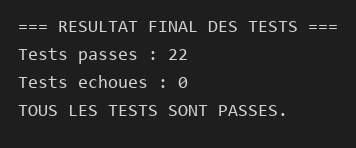
\includegraphics[width=0.82\textwidth]{figures/bilan-tests.png}%
}{%
\fbox{\parbox{0.82\textwidth}{\centering\vspace{0.6em}
Capture à coller : dernières lignes de la console,\\
bloc « RESULTAT FINAL DES TESTS »,\\
« Tests passes : 22 » et « Tests echoues : 0 ».
\vspace{0.6em}}}%
}
\caption{Bilan des vingt-deux comparaisons.}
\label{fig:bilan}
\end{figure}

\begin{figure}[ht]
\centering
\IfFileExists{figures/cours-14-16.png}{%
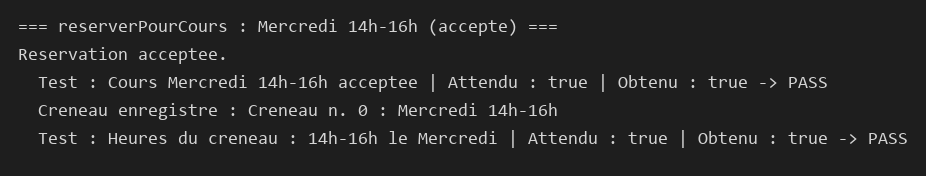
\includegraphics[width=0.82\textwidth]{figures/cours-14-16.png}%
}{%
\fbox{\parbox{0.82\textwidth}{\centering\vspace{0.6em}
Capture à coller : scénario « Mercredi 14h-16h »,\\
ligne du créneau enregistré (jour, 14\,h, 16\,h)\\
et verdict de réussite sur les heures.
\vspace{0.6em}}}%
}
\caption{Heures de cours réellement enregistrées.}
\label{fig:cours}
\end{figure}

\begin{figure}[ht]
\centering
\IfFileExists{figures/doublon-catalogue.png}{%
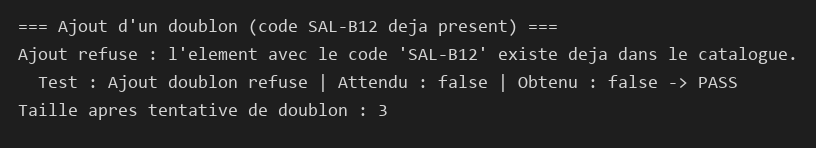
\includegraphics[width=0.82\textwidth]{figures/doublon-catalogue.png}%
}{%
\fbox{\parbox{0.82\textwidth}{\centering\vspace{0.6em}
Capture à coller : scénario d'ajout du code déjà présent,\\
message de refus et taille du catalogue inchangée,\\
avec le verdict « ajout doublon refusé ».
\vspace{0.6em}}}%
}
\caption{Second ajout du même code refusé.}
\label{fig:doublon}
\end{figure}

À côté de cette recette manuelle, le dépôt contient dix-huit tests JUnit exécutables, répartis dans \texttt{ReservationReglesTest}, \texttt{ReservationEtatTest} et \texttt{CatalogueCoursTest}. Ils vérifient les mêmes règles sans se contenter d'un affichage : créneau invalide, code vide, durée, occupation, état inchangé après refus, libération, matériel mobile, poste, doublon de catalogue, recherche, cours sans jour, cours du mercredi de 14\,h à 16\,h. La commande est dans le README. L'exécution de référence de cette suite donne dix-huit réussites et zéro échec.

Cette vérification a deux limites. Les données de la démonstration sont fixes (salle B12, projecteur, poste, deux utilisateurs) et il n'y a pas de saisie au clavier. Nous ne montrons donc pas qu'un utilisateur pourrait composer librement un créneau. Nous montrons que, sur ce jeu d'essais, les règles de durée, d'occupation, d'unicité et d'heures de cours sont celles qui ont été annoncées.

Le compte de vingt-deux réussites recouvre davantage de comparaisons que de blocs affichés. Une même situation produit souvent deux verdicts : la réponse de la réservation, puis le contrôle que l'état n'a pas bougé. C'est le cas du refus de dix heures, du jour vide, de la seconde réservation de cours et du conflit sur la salle déjà prise. D'autres comparaisons portent sur des objets : la recherche du code de la salle B12 doit retrouver l'élément déjà catalogué, et la recherche d'un code inconnu ou vide doit ne rien retrouver. Le message final de la console résume ces comparaisons ; il ne remplace pas la lecture ligne à ligne du tableau.

Pour lire un verdict, il suffit de trois informations affichées à la suite : le nom du scénario, la valeur attendue et la valeur obtenue. Lorsque les deux valeurs coïncident, la ligne est une réussite. Lorsque le contrôle porte sur l'état, la réussite signifie que la disponibilité et la réservation active sont restées celles d'avant la tentative. Un échec aurait indiqué que le programme a modifié l'élément alors que la demande devait être ignorée. Sur la version~\texttt{version-1.0}, aucune ligne de ce type n'est un échec. Le dépôt permet de relancer \texttt{Main} et de retrouver le même bilan.

\section{Bilan et perspectives}

La version finale répond au problème posé dans le périmètre choisi. Un même contrat traite la salle, le matériel mobile et le poste. Les listes rendent le catalogue et l'historique explicites. Un refus contrôlé ne laisse pas l'élément dans un autre état. Les tags \texttt{jalon-1}, \texttt{jalon-2}, \texttt{jalon-3} et \texttt{version-1.0} permettent de retrouver les étapes sur le dépôt.

Trois suites restent hors de cette version. La persistance enregistrerait le catalogue après l'arrêt du programme. Un menu permettrait de saisir un jour et des heures sans modifier le source. Une administration distinguerait l'ajout durable d'une ressource et la simple réservation. Aucune de ces trois pistes n'est livrée dans \texttt{version-1.0}.

Le point acquis est plus précis que la simple existence d'un programme qui « réserve ». Nous savons quelle demande est acceptée, laquelle est refusée, et dans quel état l'élément reste après le refus. Cette précision vient des essais, pas d'une promesse du README. C'est elle que le tag \texttt{version-1.0} permet de rejouer.

\section{Contributions et traçabilité}

Le dépôt est collectif. Les paragraphes suivants décrivent des responsabilités techniques visibles dans le README et dans l'historique Git. Ils ne reprennent pas les appréciations confidentielles de la matrice d'équipe.

NIKIEMA KAFONO ARMAND RAMZIE ARCHAD a introduit l'interface \texttt{Reservable}. C'est le contrat qui permet ensuite de manipuler une salle, un matériel et un poste sans dupliquer les opérations de réservation, de libération et d'affichage. Sans cette interface, le catalogue ne pourrait pas regrouper des types différents, et le programme principal devrait connaître chaque classe concrète. Pour le jalon~4, il a aussi préparé la section de version finale du README (lien du dépôt, tag \texttt{version-1.0}, commande de lancement, périmètre) et aligné le diagramme PlantUML sur le code livré : méthode de code, recherche par code, service de réservation et réservation de cours. Le diagramme n'est donc pas un schéma antérieur resté en retard sur les collections.

KOARA Dorianne a conçu \texttt{PosteTravail} comme élément réservable qui n'hérite pas de \texttt{Ressource}. Le point technique est de montrer qu'une interface ne sert pas seulement à factoriser deux sous-classes : elle accepte un troisième type, avec son propre code, sa zone et une durée maximale de trois heures, tout en restant compatible avec le catalogue et avec une réservation. Elle a aussi documenté le choix écarté, celui qui consistait à recopier \texttt{reserver} et \texttt{liberer} dans chaque classe, et elle a mis à jour le diagramme de classes lorsque cette relation a été introduite. Le README lui attribue explicitement le poste, le choix écarté et le diagramme.

ZERBO JUDICAEL a fait passer les essais de la salle et du matériel mobile par une référence de type \texttt{Reservable}, afin que le test ne dépende pas de la classe concrète. Il a centralisé, dans la ressource, le refus d'une durée excessive et le refus d'une ressource déjà occupée, pour que ces deux règles ne soient pas réécrites dans chaque fille. Il a ensuite ajouté le service de réservation, utilisé à la fois par la démonstration et par la réservation de cours, et la vérification qu'un échec ne change pas l'état. Après le retour de suivi, il a fait enregistrer le jour et les heures réelles, refuser le doublon de code, et afficher pour chaque scénario le résultat attendu à côté du résultat obtenu. Le bilan de vingt-deux réussites et zéro échec est celui de cette démonstration.

Le dépôt public est \url{https://github.com/Ed-sudo-collab/poo-RESFLOW-groupe2}. La chaîne des tags est \texttt{jalon-1}, puis \texttt{jalon-2}, puis \texttt{jalon-3}, puis \texttt{version-1.0}. Ce dernier tag est celui du rendu de code du jalon~4.

\section{Références et outils utilisés}

\begin{itemize}
\item Java, langage de l'application console.
\item Git et GitHub, historique et tags de jalon.
\item PlantUML, source du diagramme (\texttt{docs/diagramme.puml}).
\item Compilation et exécution par \texttt{javac} et \texttt{java}.
\item LaTeX, pour ce rapport.
\item Beamer, pour la présentation remise à part.
\item Moodle, pour les consignes, les PDF et la matrice d'équipe.
\end{itemize}

\appendix
\section{Diagramme de classes}
Le schéma annoté est dans le dépôt : \texttt{docs/Diagrammes de classes.png}. On peut le placer sous \texttt{figures/diagramme.png} pour l'insérer ici lors d'une compilation ultérieure.

\section{Journal d'exécution}
Un extrait de console, limité au bilan et au créneau de cours, peut être collé dans cette annexe. Il ne remplace pas le tableau~\ref{tab:essais}.

\end{document}
